%% generato automaticamente da tools/build_tex.py --- non modificare
\chapter{L'arcotangente attraversa il taglio}
\label{cap:atan}
\quaderno{atan.dfw}{28 Jan 2010}{14}

Gennaio 2010. Quattordici espressioni che partono da un'identità nota e la seguono fuori dal territorio in cui è nata. L'identità è che $\mathrm{e}^{\mathrm{i}\arctan x}$ è il numero complesso $1+\mathrm{i}x$ normalizzato; la domanda del quaderno è che cosa ne resti quando all'argomento reale si sostituisce un argomento immaginario. La risposta passa per il punto di diramazione dell'arcotangente e per il logaritmo complesso.

\section{Il punto di partenza}

La prima riga contiene tre scritture della stessa cosa, ed è l'osservazione su cui poggia tutto il resto: l'arcotangente di $x$ è l'argomento del numero complesso $1+\mathrm{i}x$.

\begin{espr}{1}{User}{}
\[
\mathrm{e}^{\mathrm{i}\, \arctan\!\left(x\right)} = \frac{1 + \mathrm{i}\, x}{\sqrt{x^{2} + 1}} = \operatorname{sgn}\!\left(1 + \mathrm{i}\, x\right)
\]
\end{espr}
Tre scritture equivalenti. L'identità è esatta per ogni $x$ reale; il verificatore automatico non le assegna il segno di spunta perché lo prova su punti complessi, dove l'arcotangente cambia ramo.

\begin{figure}[htbp]
  \centering
  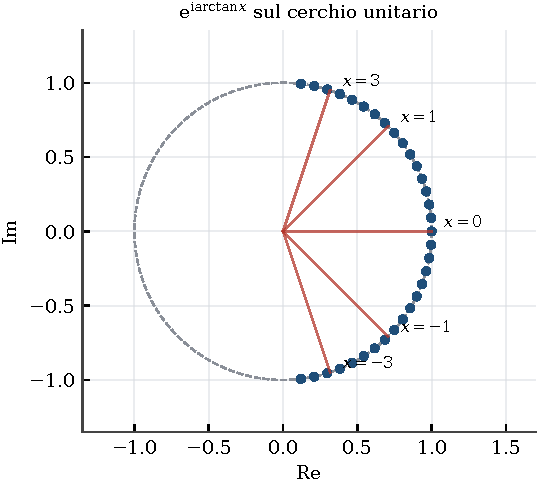
\includegraphics[width=0.58\linewidth]{../figures/atan_cerchio.pdf}
  \caption{L'identità $\#1$ in figura: al variare di $x$ reale il punto $(1+\mathrm{i}x)/\sqrt{1+x^2}$ percorre il semicerchio destro, e il suo argomento è $\arctan x$. Gli estremi $x\to\pm\infty$ corrispondono ai due punti $\pm\mathrm{i}$, che non vengono mai raggiunti.}
  \label{fig:atan_cerchio}
\end{figure}
\begin{espr}{2}{User}{\verificata}
\[
\mathrm{e}^{\mathrm{i}\, \arctan\!\left(\mathrm{i}\, x\right)} = \frac{1 - x}{\sqrt{1 - x^{2}}}
\]
\end{espr}
La sostituzione $x\to\mathrm{i}x$. Il secondo membro è $\sqrt{(1-x)/(1+x)}$ scritto senza radice al numeratore.


L'ultima delle tre scritture usa la funzione segno nel senso in cui Derive la estende ai complessi: $\mathrm{sgn}(z)=z/|z|$, cioè la proiezione sul cerchio unitario. Dire che $\mathrm{e}^{\mathrm{i}\arctan x}=\mathrm{sgn}(1+\mathrm{i}x)$ è dire che l'esponenziale immaginario è la fase, e nient'altro.

La riga $\#2$ compie il passo decisivo sostituendo $x\to\mathrm{i}x$. Poiché $\arctan(\mathrm{i}x)=\mathrm{i}\,\mathrm{artanh}(x)$, il primo membro diventa $\mathrm{e}^{-\mathrm{artanh}(x)}=\sqrt{\frac{1-x}{1+x}}$, che è esattamente il secondo membro riscritto. L'esponenziale immaginario è diventato un esponenziale reale: la rotazione si è trasformata in una dilatazione.

\section{Il punto di diramazione}

Che cosa succede esattamente in $x=1$, cioè quando l'argomento immaginario raggiunge $\mathrm{i}$?

\begin{espr}{3}{User}{}
\[
\arctan\!\left(\mathrm{i}\right) = \mathrm{i}\, \infty
\]
\end{espr}
Il punto di diramazione dell'arcotangente. La notazione $\mathrm{i}\infty$ indica una divergenza lungo l'asse immaginario.

\begin{espr}{4}{User}{}
\[
\mathrm{e}^{\mathrm{i}\, \arctan\!\left(\mathrm{i}\right)} = 0
\]
\end{espr}
Di conseguenza l'esponenziale si annulla: $\mathrm{e}^{-\infty}=0$.


L'arcotangente ha due punti di diramazione, in $\pm\mathrm{i}$, e lì diverge. Derive lo dice nel modo più diretto possibile: $\arctan(\mathrm{i})=\mathrm{i}\infty$. L'esponenziale corrispondente, avendo esponente reale negativo infinito, vale zero. È il collasso del cerchio unitario in un punto.

\section{La forma logaritmica e il ramo principale}

Le sei espressioni seguenti sviluppano l'arcotangente immaginaria in forma logaritmica e ne seguono le conseguenze passo per passo. È la parte più delicata del quaderno, perché è dove i rami del logaritmo entrano in gioco.

\begin{espr}{5}{User}{\verificata}
\[
\arctan\!\left(\mathrm{i}\, x\right) = -\frac{\pi}{2} + \frac{\mathrm{i}}{2}\, \left(\ln\!\left(x + 1\right) - \ln\!\left(x - 1\right)\right)
\]
\end{espr}
Lo sviluppo logaritmico dell'arcotangente immaginaria, nella forma valida per $x>1$. Il termine $-\pi/2$ è il contributo del ramo principale.

\begin{espr}{6}{User}{\verificata}
\begin{align*}
& \mathrm{i}\, \arctan\!\left(\mathrm{i}\, x\right) \\
=\;& -\frac{1}{2}\, \left(\ln\!\left(x + 1\right) - \ln\!\left(x - 1\right)\right) - \frac{\mathrm{i}\, \pi}{2}
\end{align*}
\end{espr}
Moltiplicata per $\mathrm{i}$: la parte immaginaria e quella reale si scambiano di ruolo.

\begin{espr}{7}{User}{\verificata}
\begin{align*}
& \mathrm{e}^{\mathrm{i}\, \arctan\!\left(\mathrm{i}\, x\right)} \\
=\;& \mathrm{e}^{-\frac{1}{2}\, \left(\ln\!\left(x + 1\right) - \ln\!\left(x - 1\right)\right) - \frac{\mathrm{i}\, \pi}{2}}
\end{align*}
\end{espr}
L'esponenziale della riga precedente.

\begin{espr}{8}{User}{\verificata}
\begin{align*}
& \mathrm{e}^{-\frac{1}{2}\, \left(\ln\!\left(x + 1\right) - \ln\!\left(x - 1\right)\right)}\, \mathrm{e}^{\frac{-\mathrm{i}\, \pi}{2}} \\
=\;& -\mathrm{i}\, \mathrm{e}^{-\frac{1}{2}\, \left(\ln\!\left(x + 1\right) - \ln\!\left(x - 1\right)\right)}
\end{align*}
\end{espr}
Il fattore $\mathrm{e}^{-\mathrm{i}\pi/2}$ vale $-\mathrm{i}$ e viene portato fuori.

\begin{espr}{9}{User}{\verificata}
\[
\mathrm{e}^{-\frac{1}{2}\, \left(\ln\!\left(x + 1\right) - \ln\!\left(x - 1\right)\right)} = \frac{\sqrt{x - 1}}{\sqrt{x + 1}}
\]
\end{espr}
Il fattore restante si semplifica in una radice: $\mathrm{e}^{-\frac12\ln\frac{x+1}{x-1}}=\sqrt{\frac{x-1}{x+1}}$.

\begin{espr}{10}{User}{\verificata}
\[
\mathrm{e}^{\mathrm{i}\, \arctan\!\left(\mathrm{i}\, x\right)} = \frac{1}{\mathrm{i}}\, \left(\frac{\sqrt{x - 1}}{\sqrt{x + 1}}\right)
\]
\end{espr}
Mettendo insieme: l'esponenziale vale la radice divisa per $\mathrm{i}$.


La riga $\#5$ merita un commento. La formula scolastica sarebbe $\arctan(\mathrm{i}x)=\tfrac{\mathrm{i}}{2}\ln\frac{1+x}{1-x}$, valida per $|x|<1$. Quella scritta qui usa invece $\ln(x-1)$ al posto di $\ln(1-x)$, e compensa con il termine costante $-\pi/2$. Non è un errore: è la continuazione analitica oltre il punto di diramazione, cioè la forma valida per $x>1$, dove $\ln(x-1)$ è reale e la scelta del ramo principale di Derive — dichiarata nell'intestazione del file con $\mathtt{Branch{:}{=}Principal}$ — aggiunge quel $-\pi/2$. Le righe successive riducono l'esponenziale a $\sqrt{(x-1)/(x+1)}$ diviso per $\mathrm{i}$, che è la controparte per $x>1$ della radice $\sqrt{(1-x)/(1+x)}$ trovata alla riga $\#2$ per $|x|<1$.

\section{La verifica per via inversa}

Le ultime quattro righe rifanno il conto al contrario: invece di sviluppare l'arcotangente, si pone l'esponenziale uguale al risultato e si risolve per l'esponente.

\begin{espr}{11}{User}{}
\[
\mathrm{e}^{z} = \frac{1 - x}{\sqrt{1 - x^{2}}}
\]
\end{espr}
Si riparte dal risultato della riga $\#2$ e lo si pone uguale a $\mathrm{e}^z$, per ricavare $z$.

\begin{espr}{12}{Simp(Solve(\#11,z))}{}
\begin{align*}
& z = -\frac{\ln\!\left(1 - x^{2}\right)}{2} + \ln\!\left(1 - x\right) - 2\, \pi\, \mathrm{i} \\[3pt]
\lor\quad & z = -\frac{\ln\!\left(1 - x^{2}\right)}{2} + \ln\!\left(1 - x\right) + 2\, \pi\, \mathrm{i} \\[3pt]
\lor\quad & z = \ln\!\left(1 - x\right) - \frac{\ln\!\left(1 - x^{2}\right)}{2}
\end{align*}
\end{espr}
Le tre soluzioni di Derive differiscono per multipli di $2\pi\mathrm{i}$: sono rami distinti dello stesso logaritmo.

\begin{espr}{13}{User}{}
\[
z = \ln\!\left(1 - x\right) - \frac{\ln\!\left(1 - x^{2}\right)}{2}
\]
\end{espr}
Il ramo principale, quello senza termine immaginario aggiunto.

\begin{espr}{14}{User}{\verificata}
\[
\mathrm{i}\, \arctan\!\left(\mathrm{i}\, x\right) = \ln\!\left(1 - x\right) - \frac{\ln\!\left(1 - x^{2}\right)}{2}
\]
\end{espr}
La conclusione: $\mathrm{i}\arctan(\mathrm{i}x)=\ln(1-x)-\tfrac12\ln(1-x^2)$, che è $-\mathrm{artanh}(x)$ scritto per esteso.


Fra le tre soluzioni che Derive restituisce alla riga $\#12$, due differiscono dalla terza per multipli di $2\pi\mathrm{i}$: sono i rami del logaritmo complesso, che il programma elenca tutti perché nessuno è privilegiato dall'equazione. La riga $\#13$ sceglie quello principale e la riga $\#14$ conclude, chiudendo il cerchio con la riga $\#2$.

\section*{In sintesi}
\addcontentsline{toc}{section}{In sintesi}

Il quaderno segue una funzione elementare fuori dal suo dominio naturale e registra con precisione che cosa le accade: l'esponenziale immaginario diventa reale, il cerchio unitario si apre in una semiretta, e in $x=1$ tutto collassa in un punto. Le righe da $\#5$ a $\#10$ sono un esercizio di contabilità dei rami del logaritmo condotto senza errori, il che con un sistema di calcolo simbolico non è mai scontato. Visto dall'altro lato, il risultato è la formula $\mathrm{e}^{s}=\left(1+\tanh\tfrac s2\right)/\left(1-\tanh\tfrac s2\right)$: la stessa tangente del semiangolo che in \dfw{gauss.dfw} produce la gaussiana, come mostra la nota a corredo di questa edizione.

